% Six things a model can do about uncertainty, and where the course did each.
%
% Single source for the diagram in optimization-private/lecture-notes/lectures/
% optimization-in-context.tex, which \input's this file via \figsrc. `make` also
% renders ../media/figures/uncertainty-responses.{png,svg} for the website.
%
% WHY THE CODA NEEDS THIS PICTURE. The closing lecture states the list twice and
% never draws it:
%
%   "Across the semester we met several responses to uncertainty: ignore it
%    (deterministic optimization, most of Part I), explore it (sensitivity
%    analysis, via the multipliers), learn it (parameter estimation), reduce it
%    (experimental design), and model it (stochastic programming). There is a
%    sixth --- protect against it."       [\subsection*{What this course did not cover}]
%
%   "Uncertainty can be ignored, explored, learned, reduced, modeled, or
%    protected against."                  [\subsection*{Six things to take with you}]
%
% Prose can only give the six in sequence. What it cannot do is show that they
% form ONE ordered spectrum, that five of the six are lectures the student has
% already sat through, and that the sixth --- the one the lecture spends a
% paragraph declining to teach --- is the far end of that same spectrum rather
% than a separate subject. That is a shape, and a shape wants a drawing. The
% whole rhetorical move of the coda is "here is the map of the semester", so
% this is the coda's map.
%
% ORDERING is the lecture's own, not invented here, and it is not arbitrary:
% reading left to right, the model is asked to do progressively more about the
% uncertainty, from acknowledging none of it to guaranteeing feasibility under
% all of it.
%
% ⚠ LECTURE NAMES, NOT LECTURE NUMBERS. main-body.tex sets \autolecturenumtrue,
% so numbers are derived from position in the pack and any number printed inside
% a figure would be stale the first time a lecture moves. The bottom row
% therefore names lectures by title, exactly as the coda's own cross-references
% do.
%
% ⚠ RE-VERIFIED 2026-09-17 against \lecture{}{} in each source file, and FOUR OF
% THE FIVE ENTRIES HAD DRIFTED. The list now reads:
%   introduction.tex               "Introduction: Why and How We Optimize"
%   kkt-conditions.tex             "KKT Conditions, Multipliers, and Sensitivity"
%   parameter-estimation-doe.tex   "Parameter Estimation and Experimental Design"
%   stochastic-programming-intro.tex      "Stochastic Programming: Introduction"
%   stochastic-programming-advanced.tex   "Stochastic Programming: Information and Risk"
% Shortened here for width; every short form is a prefix or an obvious contraction
% of the real title.
%
% WHAT THE OLD LIST CLAIMED, AND WHY IT IS RECORDED RATHER THAN QUIETLY
% OVERWRITTEN. Its second line read
%
%   kkt-multipliers.tex            "KKT Multipliers and Constraint Qualifications"
%
% and BOTH HALVES of that were wrong, in different ways and at different times:
%
%   * THE TITLE WAS NEVER RIGHT. The file did exist on 2026-08-19, the date the
%     old comment gives for the verification, but its own header read
%     \lecture{19}{KKT Multipliers and Sensitivity} -- checked with
%     `git show 8383c43^:lecture-notes/lectures/kkt-multipliers.tex'. So the
%     quoted title belonged to no lecture on the day it was "verified"; it looks
%     like a conflation with constraint-qualifications.tex, which is the NEXT
%     lecture and a separate file. A verification claim that was false when it
%     was written is the more useful half of this note: it is the reason to
%     re-read the source rather than trust the list.
%   * THE FILE IS NOW GONE. kkt-multipliers.tex was merged IN FULL into
%     lectures/kkt-conditions.tex on 2026-08-21 with Prof. Dowling's approval,
%     and deleted; optimization-private/lecture-notes/main-body.tex carries the
%     merge header and the recovery command.
%
% THE PICTURE'S CLAIM ITSELF STILL HOLDS, which is why this is repointed and not
% withdrawn: the lecture that now teaches rung 2 is kkt-conditions.tex, whose
% \goal IS the sensitivity derivation -- "Derive the sensitivity interpretation
% d obj(x*)/d eps = mult*_ihat" -- so "explore" is still a response the student
% has sat through, in one lecture, under a title that names it.
%
% ⚠ THE DRAWN LABEL ON RUNG 2 STILL READS "KKT Multipliers", which is no longer
% a prefix or a contraction of the real title -- it is the old lecture's name.
% Deliberately NOT changed here: the label is rendered output
% (../media/figures/uncertainty-responses.{png,svg} would have to be rebuilt,
% and figures/Makefile rebuilds everything), and it is already tracked as a
% \fixnote in Lecture 27 by the L26/L27 audit of 2026-09-17, which proposes
% "KKT Conditions \& Sensitivity". This comment fixes the AUDIT TRAIL; the label
% is Prof. Dowling's call and is flagged where he will see it, in the PDF.
%
% GREYSCALE. Nothing is encoded by hue -- the file contains no colour at all.
% The five taught responses are SOLID black boxes; the untaught sixth is DASHED
% and grey AND carries the words "not covered". Either the line style or the
% text carries the contrast alone, so the figure is identical on a mono laser
% printer. This follows the house precedent set by decision-loop.tex and
% scenario-tree.tex, whose headers record why a blue diagram fails
% scripts/check_greyscale.py in image mode: a thin coloured stroke antialiases
% into a family of near-identical tones that the checker reports as colliding
% series. Black and grey blend only into greys.

% `positioning' is loaded HERE rather than in the course-pack preamble so this
% file is self-contained: the same source is \input by the lecture and built
% standalone by figures/Makefile. \usetikzlibrary is idempotent, so loading it
% twice is harmless. See the same note in scenario-tree.tex.
\usetikzlibrary{positioning}

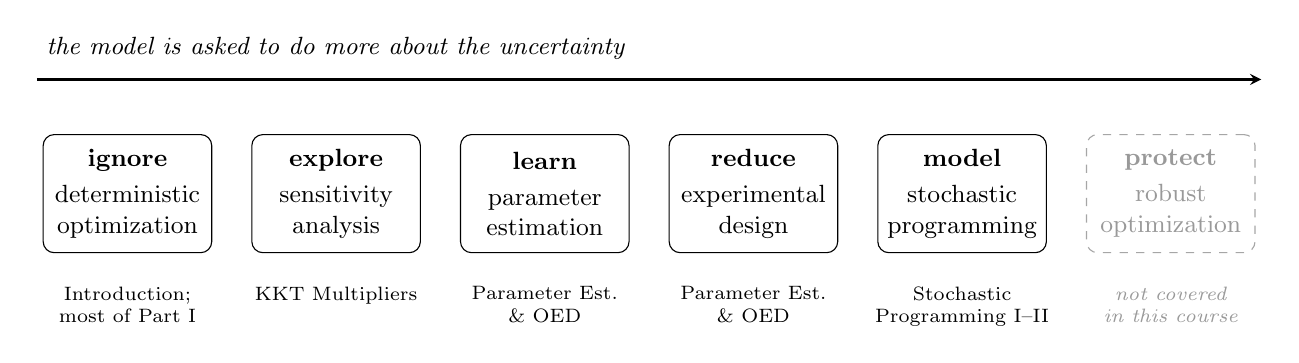
\begin{tikzpicture}[>=stealth, font=\small,
    % NB: `step' and `where' are NOT available as style names -- /tikz/step is
    % the built-in grid spacing key, and using it here fails with the unhelpful
    % "the key '/tikz/step' requires a value". Hence the rung* names.
    rung/.style={draw=black, fill=white, rounded corners,
                 minimum height=15mm, text width=20mm, align=center,
                 inner sep=2pt, font=\small},
    runggone/.style={draw=gray!70, dashed, fill=white, rounded corners,
                   minimum height=15mm, text width=20mm, align=center,
                   inner sep=2pt, font=\small, text=gray!80},
    rungwhere/.style={font=\scriptsize, align=center, text width=23mm},
    runggonelab/.style={font=\scriptsize\itshape, align=center, text width=23mm,
                 text=gray!80}]

  % ---- the six responses, left to right: the model does progressively more
  \node[rung]   (s1) at (0.00,0) {\textbf{ignore}\\[2pt]deterministic\\optimization};
  \node[rung]   (s2) at (2.65,0) {\textbf{explore}\\[2pt]sensitivity\\analysis};
  \node[rung]   (s3) at (5.30,0) {\textbf{learn}\\[2pt]parameter\\estimation};
  \node[rung]   (s4) at (7.95,0) {\textbf{reduce}\\[2pt]experimental\\design};
  \node[rung]   (s5) at (10.60,0) {\textbf{model}\\[2pt]stochastic\\programming};
  \node[runggone] (s6) at (13.25,0) {\textbf{protect}\\[2pt]robust\\optimization};

  % ---- where each one was taught (or, for the sixth, was not)
  \node[rungwhere, below=3mm of s1] {Introduction;\\most of Part~I};
  \node[rungwhere, below=3mm of s2] {KKT Multipliers};
  \node[rungwhere, below=3mm of s3] {Parameter Est.\\ \& OED};
  \node[rungwhere, below=3mm of s4] {Parameter Est.\\ \& OED};
  \node[rungwhere, below=3mm of s5] {Stochastic\\Programming I--II};
  \node[runggonelab, below=3mm of s6] {not covered\\in this course};

  % ---- the spectrum the six sit on
  \draw[->, thick, draw=black] (-1.15,1.45) -- (14.40,1.45);
  \node[font=\small\itshape, anchor=west] at (-1.15,1.85)
    {the model is asked to do more about the uncertainty};
\end{tikzpicture}
